\newpage
\section{Minutes of Meeting}

\subsection{Project Kick-Off}
\label{appendix:kick_off_mom}

\momtoptable
{Fri 12-Jan 2018 (Week 1)}
{Boyd Orr}
{Christopher Bellingham}
{Ioannis Athanasiadis [IA]\newline
Christopher Bellingham [CB]\newline
Joseph Doogan [JD]\newline
Pavlos Evangelidis [PE]\newline
Torquil MacLeod [TM]}
{-}

\begin{momitems}
	% Item, Details, Resp., Due.
	\momitem
	{1}
	{Team reviewed and approved Team Organisation Document.}
	{INFO}
	{INFO}

	\momitem
	{2}
	{Publish latest Team Organisation Document to Slack to allow each team member to submit to Moodle.}
	{CB}
	{Fri 12-Jan}

	\momitem
	{3}
	{Create Customer Specification, capturing all requirements. Post-meeting note, see Appendix \ref{appendix:customer_specification}.}
	{CB}
	{Sun 14-Jan}

	\momitem
	{4}
	{Populate Trello with User Stories based on Customer Spec prior to Sprint Planning meeting on Wed-17.}
	{ALL}
	{Wed 17-Jan}

	\momitem
	{5}
	{Consider architecture and high-level Object Orientated design prior to Design meeting on Wed-17.}
	{ALL}
	{Wed 17-Jan}
\end{momitems}


\newpage
\subsection{Sprint Planning Meeting}
\label{appendix:sprint1_planning_meeting}

\momtoptable
{Wed 17-Jan 2018 (Week 2)}
{Slack}
{Christopher Bellingham}
{Ioannis Athanasiadis [IA]\newline
Christopher Bellingham [CB]\newline
Joseph Doogan [JD]\newline
Pavlos Evangelidis [PE]\newline
Torquil MacLeod [TM]}
{-}

\begin{momitems}
	% Item, Details, Resp., Due.
	\momitem
	{1}
	{User stories submitted to Trello were reviewed. Duplicate stories were eliminated, remaining stories were allocated durations.}
	{INFO}
	{INFO}
	
	\momitem
	{2}
	{Unique Story IDs were granted to each User Story, in the form SXXXX. This will aid communication as development progresses.}
	{INFO}
	{INFO}

	\momitem
	{3}
	{Team agreed to define each story as a Must Have, since all generated stories are strictly limited to the requirements of the specification. The team reserves the right to de-prioritise individual stories should the workload be considered too high.}
	{INFO}
	{INFO}

	\momitem
	{4}
	{The sum of all story points is 16. Broadly, Team feels development can be split into two main phases - command line mode, and online mode. Resultant stories can be found in Appendix \ref{appendix:user_stories_command_line} and Appendix \ref{appendix:user_stories_online} respectively.}
	{INFO}
	{INFO}

	\momitem
	{5}
	{Command line mode covers stories S0010, S0020, S0030, S0040, S0050, S0130, S0180. This equates to a total of 9 story points.}
	{INFO}
	{INFO}

	\momitem
	{6}
	{Online mode covers stories S0190, S0200, S0210, S0220, S0230, S0240, S0250. This equates to a total of 7 story points.}
	{INFO}
	{INFO}

	\momitem
	{7}
	{Development of command line and online mode will be tackled over the course of two 1-week long sprints. With consideration for the need for sprint planning/retrospectives, this leaves 6 days per sprint. Each team member's capacity was assumed to be one third of this duration, I.e. 2 ideal days each. Considering a team size of 5, total available capacity per sprint is 10 ideal days.}
	{INFO}
	{INFO}

	\momitem
	{8}
	{With consideration of team capacity, it is deemed feasible to tackle the project over the course of two 1-week sprints. Sprint 1 will tackle command line mode. Sprint 2 will tackle online mode.}
	{INFO}
	{INFO}

	\momitem
	{9}
	{With initial consideration to an MVC-style architecture, it was noted that each story may slice through multiple layers of this architecture. Team considers it sensible for individuals to have responsibility over different segments of the system, as such each user story will be split between multiple developers. Allocation of user stories to individuals will therefore be deferred until this afternoon's design meeting, where architecture and class structure will be finalised.}
	{INFO}
	{INFO}

	\momitem
	{10}
	{Project schedule was created, allowing for 6-days float/contingency prior to report submission (Figure \ref{figure:initial_project_plan}).}
	{INFO}
	{INFO}

	\momitem
	{11}
	{It was agreed that the requirements presented in Appendix \ref{appendix:customer_specification} should be cross-referenced to each user story, to ensure full coverage of requirements. A coverage matrix will be produced by the team to confirm there are no coverage gaps.}
	{ALL}
	{Fri 19-Jan}
\end{momitems}

\begin{center}
	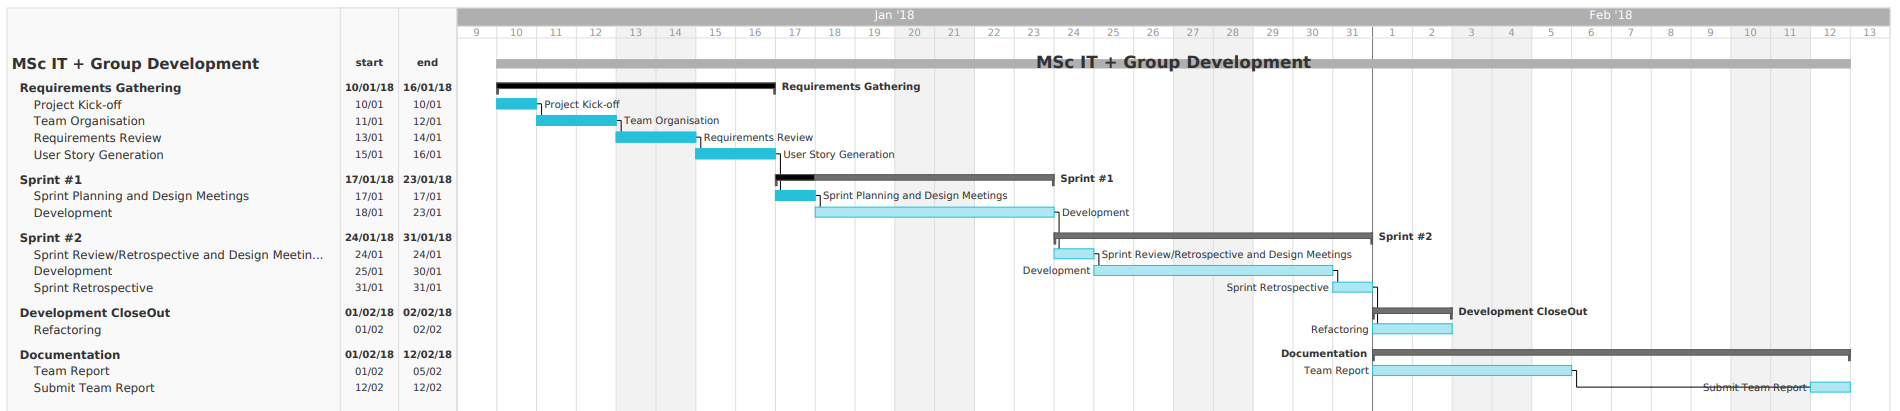
\includegraphics[scale=0.35, angle=90]{initial_project_plan}
	\captionof{figure}{Initial Project Plan}
	\label{figure:initial_project_plan}
\end{center}

\newpage
\subsection{System Design Meeting}

\momtoptable
{Wed 17-Jan 2018 (Week 2)}
{Slack}
{Christopher Bellingham}
{Ioannis Athanasiadis [IA]\newline
Christopher Bellingham [CB]\newline
Joseph Doogan [JD]\newline
Pavlos Evangelidis [PE]\newline
Torquil MacLeod [TM]}
{-}

\begin{momitems}
	% Item, Details, Resp., Due.
	\momitem
	{1}
	{CB provided a candidate architecture diagram (Figure \ref{figure:initial_architecture}), outlining use of an MVC architecture, with a data persistence layer. CB proposed use of the Observer Pattern as a means of reducing coupling between MVC layers.}
	{INFO}
	{INFO}

	\momitem
	{2}
	{Use of the Observer Pattern was identified as a risk, since no team member has experience with this. CB will outline how this would work by providing an example of a simple implementation.}
	{CB}
	{Wed 17-Jan}

	\momitem
	{3}
	{Prior to the meeting, each team member had submitted class diagrams to enable discussion on needed class structures. Each submission was reviewed, and it was noted that a lot of commonality exists across proposed classes (typically Game, Player and Card classes).}
	{INFO}
	{INFO}

	\momitem
	{4}
	{CB provided detailed UML covering full system (Figure \ref{figure:initial_uml}). It is understood that online mode can hook into key Game functionality via game's available public methods, and online components can be notified of game state changes via the Observer mechanism. The approach as depicted was agreed to be a reasonable solution, and was selected as a basis for overall design.}
	{INFO}
	{INFO}

	\momitem
	{5}
	{CB provided detailed sequence diagram covering logical flow for command line mode (Figure \ref{figure:initial_sequence_diagram}). This may be used as a reference during development.}
	{INFO}
	{INFO}

	\momitem
	{6}
	{User stories allocated to team to allow development to commence.}
	{INFO}
	{INFO}
\end{momitems}

\begin{center}
	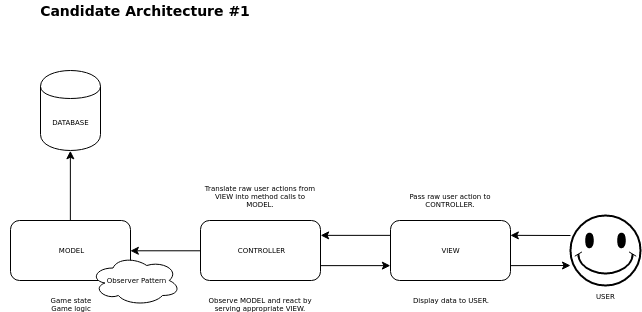
\includegraphics[scale=0.7]{initial_architecture}
	\captionof{figure}{Proposed Architecture}
	\label{figure:initial_architecture}
\end{center}

\begin{center}
	\missingfigure{Include UML with Joe's updates.}
	\captionof{figure}{Proposed UML}
	\label{figure:initial_uml}
\end{center}

\begin{center}
	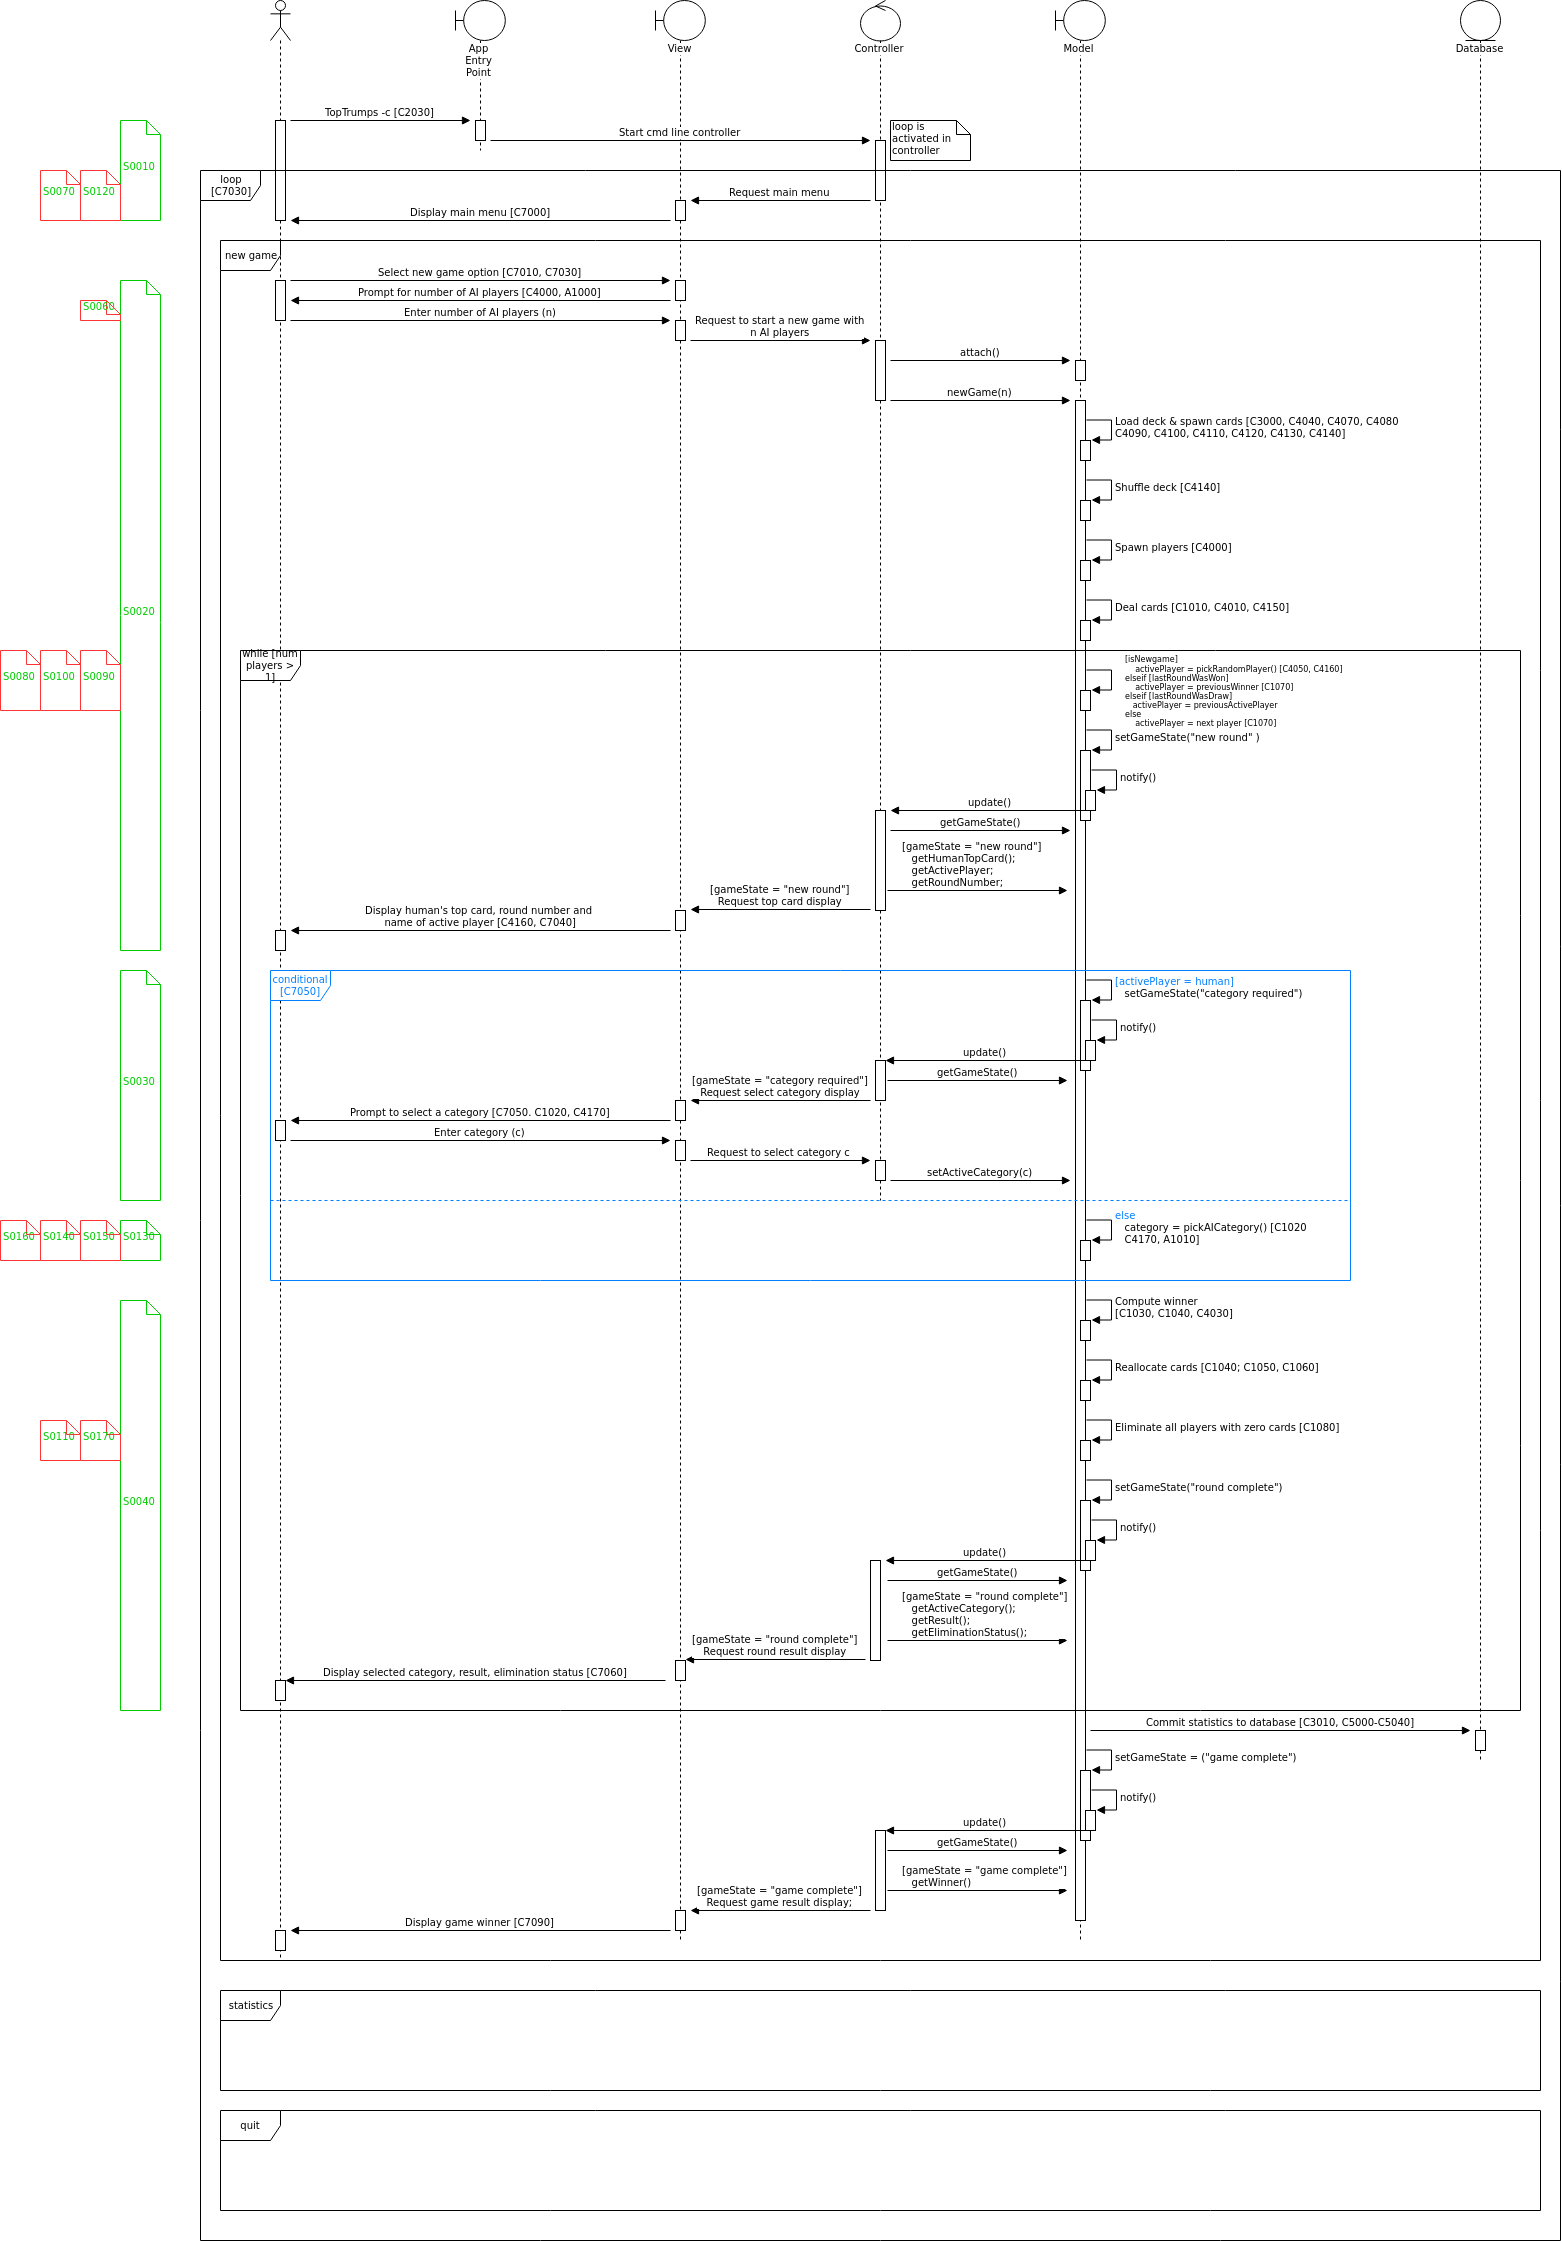
\includegraphics[scale=0.25]{initial_sequence_diagram}
	\captionof{figure}{Proposed Logical Flow}
	\label{figure:initial_sequence_diagram}
\end{center}
